\documentclass{crm-article}

% Compatibility of the journal's citehack with extended labels produced by
% current LaTeX packages.  Without this patch, a reference may contain its
% internal hyperlink anchor, for example ``3.3equation.3.3''.
\makeatletter
\def\CRMfirstoffields#1#2#3\null{#1}
\def\CRMsecondoffields#1#2#3\null{#2}
\renewcommand{\ref}[1]{%
  \expandafter\let\expandafter\CRMreftemp\csname r@#1\endcsname
  \@setref\CRMreftemp\CRMfirstoffields{#1}}
\renewcommand{\pageref}[1]{%
  \expandafter\let\expandafter\CRMpagereftemp\csname r@#1\endcsname
  \@setref\CRMpagereftemp\CRMsecondoffields{#1}}
\makeatother

\begin{document}

% Для рукописи номер тома, выпуска и редакционные даты заполняет редакция.
% \journalVol{}
% \journalNo{}
\setcounter{page}{1}

\journalSection{Математические основы и численные методы моделирования}
\journalSectionEn{Mathematical modeling and numerical simulation}

\UDC{519.85:656.13}
\title{Восстановление матрицы корреспонденций по частично наблюдаемым
равновесным потокам}
\titleeng{Origin--destination matrix recovery from partially observed
equilibrium link flows}

% TODO перед подачей: заменить заглушки ФИО и добавить e-mail всех авторов.
\affiliationnoref
\author{\firstname{И.\,О.}~\surname{Фамилия А}}
\authorfull{Имя Отчество Фамилия А}
\authoreng{\firstname{I.\,O.}~\surname{Surname A}}
\authorfulleng{First Patronymic Surname A}
\affiliation{Московский физико-технический институт (национальный
исследовательский университет),\protect\\
Россия, 141701, Московская область, г. Долгопрудный,
Институтский пер., д. 9}
\affiliationeng{Moscow Institute of Physics and Technology,
9 Institutskiy per., Dolgoprudny, Moscow Region, 141701, Russia}

\author[1]{\firstname{И.\,О.}~\surname{Фамилия Б}}
\authorfull{Имя Отчество Фамилия Б}
\authoreng[1]{\firstname{I.\,O.}~\surname{Surname B}}
\authorfulleng{First Patronymic Surname B}

\author[1]{\firstname{И.\,О.}~\surname{Фамилия В}}
\authorfull{Имя Отчество Фамилия В}
\authoreng[1]{\firstname{I.\,O.}~\surname{Surname C}}
\authorfulleng{First Patronymic Surname C}

\author[1]{\firstname{И.\,О.}~\surname{Фамилия Г}}
\authorfull{Имя Отчество Фамилия Г}
\authoreng[1]{\firstname{I.\,O.}~\surname{Surname D}}
\authorfulleng{First Patronymic Surname D}

% TODO перед подачей: при наличии гранта добавить \thanks и \thankseng.

\begin{abstract}
Матрица корреспонденций задаёт объёмы поездок между парами транспортных зон и
служит исходными данными для расчёта равновесной загрузки дорожной сети. Для
её непосредственного определения необходима подробная информация о
перемещениях между зонами, тогда как на практике чаще доступны измерения
потоков лишь на отдельных участках сети. В работе рассматривается обратная
задача восстановления матрицы корреспонденций по таким частичным наблюдениям.
Зависимость равновесного потока от спроса задаётся неявно как решение выпуклой
задачи Бекмана, соответствующей равновесию Вардропа и функциям времени проезда
BPR. На внешнем уровне минимизируется сумма квадратичной невязки потоков на
наблюдаемых рёбрах и энтропийного регуляризатора. Суммарные объёмы отправлений
и прибытий считаются известными и задаются как точные ограничения.

Для приближённого вычисления градиента дифференцируется конечный алгоритм
Франк--Вульфа. Матрицы принадлежности рёбер выбранным кратчайшим путям
накапливаются одновременно с потоком и образуют аппроксимацию якобиана
равновесного назначения по элементам матрицы корреспонденций. Внешняя задача
решается методом Adam с убывающим шагом. После каждой итерации процедура
пропорционального масштабирования строк и столбцов восстанавливает
неотрицательность, нулевую диагональ и заданные маргинальные суммы.

Алгоритм исследован на сети Sioux Falls. Рассмотрены случайные множества
наблюдаемых рёбер, несколько способов размещения фиксированного числа датчиков
и наблюдение рёбер с крупнейшими потоками. Качество оценивается по ошибке
потока на всей исходной сети и по средней ошибке после удаления отдельного
ребра с сохранением связности. Вторая метрика характеризует переносимость
восстановленного спроса при изменении топологии. При малом числе датчиков
уменьшение невязки на наблюдаемых рёбрах не гарантирует точности на всей сети.
С расширением покрытия качество заметно улучшается, но перенос на изменённую
топологию остаётся более трудной задачей. Наблюдение наиболее нагруженных
рёбер эффективно при ограниченном бюджете, однако выбор только по величине
потока не универсален. Поэтому для оценки необходимы внешние диагностические
метрики, а качество восстановления зависит и от числа датчиков, и от их
расположения.
\end{abstract}

\keyword{матрица корреспонденций}
\keyword{равновесное транспортное назначение}
\keyword{двухуровневая оптимизация}
\keyword{размещение датчиков}

\begin{abstracteng}
An origin--destination (OD) matrix specifies trip volumes between pairs of
transportation zones and provides the demand input for equilibrium network
assignment. Determining it directly requires detailed information about
movements between zones, whereas in practice flow measurements are usually
available only on selected links. We study the inverse problem of recovering
an OD matrix from such partial observations. The dependence of equilibrium
flows on demand is defined implicitly by the convex Beckmann problem with BPR
travel-time functions. At the upper level, the objective combines squared flow
mismatch on observed links with an entropy regularizer. Total departures and
arrivals are treated as known and imposed as hard constraints.

To approximate the gradient, we differentiate the finite Frank--Wolfe
procedure. Link--path incidence matrices generated by its shortest-path
subproblems are accumulated together with the flow and form an approximation
of the assignment Jacobian with respect to OD entries. The upper-level problem
is solved by Adam with a decaying step. After every iteration, iterative
proportional fitting restores nonnegativity, the zero diagonal, and the
prescribed marginal totals.

The algorithm is evaluated on the Sioux Falls network. We consider random
sets of observed links, several ways of placing a fixed number of sensors, and
observation of links carrying the largest flows. Performance is measured by
the flow error on the original network and by the mean error after deleting a
link while preserving connectivity. The latter metric characterizes transfer
under a change in topology. With sparse coverage, reducing mismatch on
observed links does not guarantee accurate flows on the entire network.
Broader coverage improves recovery, but transfer to a modified topology
remains more difficult. Observing heavily loaded links is effective under a
limited budget, although selection based only on flow magnitude is not
universally preferable. External diagnostic metrics are therefore necessary,
and recovery quality depends on both the number and the location of sensors.
\end{abstracteng}

\keywordeng{OD matrix}
\keywordeng{traffic assignment}
\keywordeng{bilevel optimization}
\keywordeng{sensor placement}

\maketitle
\fancyhead[CO]{\normalfont\normalsize
\truncate{104mm}{Восстановление OD-матрицы по частичным потокам}}
\numberparagraphs
% The journal class does not reset its custom subparagraph counter.
\renewcommand{\newpar}{%
  \stepcounter{parno}\setcounter{subparno}{0}\theparno.~}

\paragraph{Введение}

Матрица корреспонденций (origin--destination matrix, OD-матрица) описывает
число поездок между транспортными зонами за фиксированный период. Она нужна
для расчёта нагрузки на сеть, оценки инфраструктурных проектов и анализа
сценариев перекрытия дорог. В отличие от потоков на отдельных участках,
которые можно регистрировать стационарными датчиками, OD-матрица не наблюдается
непосредственно. Поэтому её оценивают по косвенным данным, в частности по
счётчикам потока, решая обратную задачу транспортного назначения. При наличии
заторов доли выбора маршрутов зависят от самой матрицы спроса, и естественно
возникает двухуровневая постановка: внешний уровень изменяет спрос, а
внутренний каждый раз вычисляет равновесные потоки
\cite{Yang1992,Mohanty2020,Castiglione2021}.

Одной только малой невязки на рёбрах с датчиками недостаточно. Во-первых,
размерность OD-матрицы обычно существенно превышает число доступных счётчиков.
Во-вторых, решение должно воспроизводить потоки вне наблюдаемого множества и
сохранять содержательный смысл после локального изменения сети. Наконец,
информативность датчиков неодинакова и зависит от их положения
\cite{ZhouList2010,Dey2020}. Эти обстоятельства определяют две цели настоящей
работы: построить воспроизводимый градиентный алгоритм с жёстким учётом
маргиналий спроса и экспериментально установить, как доля и способ выбора
наблюдаемых рёбер влияют на обобщающую способность восстановленной матрицы.

Основной методический результат состоит в совместном выполнении метода
Франк--Вульфа и рекурсии для локальной чувствительности равновесного потока.
В отличие от численного дифференцирования каждой компоненты OD-матрицы,
маршрутные матрицы получаются непосредственно из уже решаемых подзадач
кратчайших путей. Внешний шаг Adam завершается IPF-проекцией на известные
исходящие и входящие суммы. Экспериментальный результат состоит в сравнении
трёх протоколов размещения датчиков и в оценке восстановления на ансамбле
сетей с удалённым ребром. Сходимость самой OD-матрицы намеренно не используется
как основной критерий: при частичных наблюдениях она слабо идентифицируема, в
то время как практическая цель состоит в воспроизведении потоков.

% TODO(literature-review): перед подачей расширить обзор современными работами,
% сопоставить статические и динамические ODME-методы и чётче отделить вклад
% статьи. Журнал КиМ требует современные международные журнальные источники.

\paragraph{Математическая постановка}

\subparagraph{Транспортная сеть и допустимый спрос}

Пусть транспортная сеть задана ориентированным графом
$G=(V,E)$, где $|V|=n$, $|E|=m$. Все вершины в рассматриваемом тесте являются
транспортными зонами. Матрица корреспонденций
$D=(D_{ij})\in\mathbb{R}^{n\times n}_{+}$ удовлетворяет $D_{ii}=0$.
Известны маргиналии
\begin{gather}
 l_i=\sum\limits_{j=1}^{n}D_{ij},\qquad
 w_j=\sum\limits_{i=1}^{n}D_{ij},
 \label{eq:marginals}
\end{gather}
то есть полные числа отправлений и прибытий по зонам. Допустимое множество
имеет вид
\begin{gather}
 \mathcal{D}(l,w)=\left\{D\in\mathbb{R}^{n\times n}_{+}:\
 D\boldsymbol{1}=l,\quad D^{\mathsf T}\boldsymbol{1}=w,\quad
 D_{ii}=0\right\}.
 \label{eq:feasible-D}
\end{gather}
Жёсткое задание маргиналий соответствует ситуации, когда агрегированные
объёмы поездок доступны из более надёжного внешнего источника, но их
распределение между парами зон неизвестно.

Для ребра $e$ время проезда зависит от потока $f_e$ по функции BPR
\cite{BPR1964}:
\begin{gather}
 t_e(f_e)=t^0_e\left[1+a_e\left(\frac{f_e}{c_e}\right)^{b_e}\right],
 \qquad c_e>0,\quad t^0_e>0,
 \label{eq:bpr}
\end{gather}
где $c_e$ --- пропускная способность, $t^0_e$ --- время свободного
проезда. В тесте Sioux Falls для всех рёбер $a_e=0.15$, $b_e=4$.

\subparagraph{Равновесное назначение}

При фиксированной матрице $D$ множество $\mathcal{F}(D)$ содержит потоки на
рёбрах, которые могут быть получены распределением каждой корреспонденции по
путям с выполнением законов сохранения. Равновесный поток Вардропа находится
как решение задачи Бекмана \cite{Beckmann1956}
\begin{gather}
 f(D)\in\mathop{\rm arg\,min}\limits_{f\in\mathcal{F}(D)}
 \Phi(f),\qquad
 \Phi(f)=\sum\limits_{e\in E}\int\limits_{0}^{f_e}t_e(s)\,ds.
 \label{eq:beckmann}
\end{gather}
Монотонность функций \eqref{eq:bpr} обеспечивает выпуклость потенциала по
$f$. При этом отображение $D\mapsto f(D)$ является нелинейным и может быть
недифференцируемым в точках смены кратчайшего пути.

\subparagraph{Внешняя целевая функция}

Пусть $\widehat f=f(D^{\rm true})$ --- референсный поток, а
$M\in\{0,1\}^{m}$ --- маска датчиков: $M_e=1$, если поток на ребре $e$
наблюдается. Внешняя постановка имеет вид
\begin{gather}
 \min\limits_{D\in\mathcal{D}(l,w)} J(D),
 \qquad
 J(D)=\frac{1}{2}\left\|M\odot\bigl(f(D)-\widehat f\bigr)\right\|_2^2
 +\gamma\sum\limits_{i\ne j}D_{ij}\bigl(\ln D_{ij}-1\bigr),
 \label{eq:outer-objective}
\end{gather}
где $\odot$ обозначает поэлементное умножение, $0\ln 0=0$, а второе
слагаемое является выпуклой отрицательной энтропией. При фиксированной сумме
элементов этот регуляризатор предпочитает более распределённые матрицы среди
решений с близкой потоковой невязкой; он не является штрафом за отклонение от
неизвестной $D^{\rm true}$. Положительность внедиагональных элементов в коде
обеспечивается отдельно численным порогом $\varepsilon=10^{-12}$ при
масштабировании IPF. Алгоритм ищет приближённое решение
\eqref{eq:outer-objective}; при фактическом вычислении $f(D)$ заменяется
результатом конечного внутреннего цикла.

\paragraph{Численный метод}

\subparagraph{Метод Франк--Вульфа и аппроксимация якобиана}

Задача \eqref{eq:beckmann} решается методом Франк--Вульфа
\cite{FrankWolfe1956}. На внутренней итерации $q$ для текущего поля времён
$t(f_{q-1})$ строятся деревья кратчайших путей из каждой зоны. Для пары
$(i,j)$ положим $\kappa(i,j)=(i-1)n+j$. Обозначим через
$A_q\in\{0,1\}^{m\times n^2}$ соответствующую матрицу маршрутизации:
\begin{gather}
 (A_q)_{e,\kappa(i,j)}=
 \begin{cases}
 1,&\text{если ребро $e$ входит в выбранный кратчайший путь $i\to j$},\\
 0,&\text{иначе}.
 \end{cases}
 \label{eq:routing-matrix}
\end{gather}
Столбец $\kappa(i,j)$ указывает рёбра единственного пути, выбранного
алгоритмом для корреспонденции $D_{ij}$. Поэтому при фиксированном дереве
кратчайших путей поток назначения ``всё или ничего'' (all-or-nothing) линеен
по $D$, а его производная по
$\mathop{\rm vec}(D)$ в точности равна $A_q$. Само назначение и шаг
Франк--Вульфа имеют вид
\begin{gather}
 y_q=A_q\mathop{\rm vec}(D),\qquad
 \rho_q=\frac{2}{q+2},\qquad
 f_q=(1-\rho_q)f_{q-1}+\rho_q y_q,
 \quad f_0=0.
 \label{eq:fw}
\end{gather}
В реализации $f_0=0$, хотя нулевой поток не принадлежит
$\mathcal{F}(D)$ при ненулевом спросе. Поэтому конечную рекурсию
\eqref{eq:fw} следует понимать как фактически используемую численную схему,
а не как последовательность допустимых точек классической схемы
Франк--Вульфа. Сумма весов назначений на выбранные кратчайшие пути после $q$
шагов равна $1-2/[(q+1)(q+2)]$ и стремится к единице.

В коде внутренний цикл заканчивается по достижении максимального числа шагов
или условия $\eta_q\leq\eta_{\rm tol}$, где фактически вычисляется
\begin{gather}
 c_q^{\rm AON}=\sum\limits_{i,j}D_{ij}
 d_{ij}\bigl(t(f_{q-1})\bigr),\qquad
 \eta_q=\frac{\left|\langle f_q,t(f_q)\rangle-c_q^{\rm AON}\right|}
 {\langle f_q,t(f_q)\rangle}.
 \label{eq:fw-stopping}
\end{gather}
Здесь $d_{ij}(t)$ --- длина кратчайшего пути при весах $t$. Это именно
реализованный критерий остановки, а не стандартный относительный двойственный
зазор Франк--Вульфа.

Зафиксируем число выполненных внутренних шагов и предположим, что выбранные
деревья кратчайших путей не меняются в некоторой окрестности текущей матрицы
$D$. Дифференцирование выпуклой комбинации \eqref{eq:fw} даёт рекурсию
\begin{gather}
 G_0=0,\qquad
 G_q=(1-\rho_q)G_{q-1}+\rho_q A_q,
 \qquad
 G_q=\frac{\partial f_q}{\partial\mathop{\rm vec}(D)}.
 \label{eq:jacobian-recurrence}
\end{gather}
Смысл рекурсии прост: $A_q$ показывает, по каким рёбрам проходит каждая
корреспонденция на текущей итерации, а $G_q$ накапливает эти маршрутные матрицы
с теми же коэффициентами, с которыми усредняется поток. Поэтому элемент
$(G_q)_{e,\kappa(i,j)}$ используется как приближение производной
$\partial f_{q,e}/\partial D_{ij}$. Якобиан вычисляется одновременно с потоком
и не требует отдельных запусков транспортного назначения для каждой пары
$(i,j)$.

Рекурсия даёт точную производную конечного внутреннего цикла только при
фиксированных числе итераций и выбранных путях. В фактическом алгоритме число
шагов определяется условием \eqref{eq:fw-stopping}, а кратчайшие пути могут
переключаться. Поэтому $G_q$ является алгоритмической аппроксимацией якобиана,
а не производной точного равновесного отображения во всех точках.

Покажем теперь, как из якобиана получается градиент. Потоковая часть целевой
функции для результата внутреннего цикла имеет вид
\begin{gather}
 J_{\rm flow}(D)=\frac12\sum\limits_{e=1}^{m}
 M_e\bigl(f_{q,e}(D)-\widehat f_e\bigr)^2.
 \label{eq:flow-objective-finite}
\end{gather}
Здесь использовано равенство $M_e^2=M_e$ для бинарной маски. Дифференцируя
сложную функцию $D_{ij}\mapsto f_{q,e}(D)\mapsto J_{\rm flow}(D)$, получаем
\begin{gather}
 \frac{\partial J_{\rm flow}}{\partial D_{ij}}
 =\sum\limits_{e=1}^{m}
 \frac{\partial J_{\rm flow}}{\partial f_{q,e}}
 \frac{\partial f_{q,e}}{\partial D_{ij}}
 \approx\sum\limits_{e=1}^{m}
 M_e\bigl(f_{q,e}-\widehat f_e\bigr)
 (G_q)_{e,\kappa(i,j)}.
 \label{eq:gradient-component}
\end{gather}
То есть сначала вычисляется остаток
$r_q=M\odot(f_q-\widehat f)$, затем произведение $G_q^{\mathsf T}r_q$
одновременно даёт все $n^2$ производных потоковой невязки. После добавления
производной отрицательной энтропии, равной $\gamma\ln D_{ij}$ при $D_{ij}>0$,
используемая в коде матричная аппроксимация градиента записывается как
\begin{gather}
 \widetilde g(D)=\mathop{\rm unvec}\bigl(G_q^{\mathsf T}r_q\bigr)
 +\gamma\ln\bigl(\max(D,\varepsilon)\bigr),
 \qquad \widetilde g_{ii}=0.
 \label{eq:outer-gradient}
\end{gather}
Максимум и логарифм в \eqref{eq:outer-gradient} понимаются поэлементно, а
$\widetilde g_{ii}=0$ соответствует фиксированной нулевой диагонали.
Ненаблюдаемые рёбра не дают вклада в потоковую часть ни целевой функции, ни её
градиентной аппроксимации.

\subparagraph{Adam и восстановление маргиналий}

Пусть $h_k=\widetilde g(D_{k-1})$, $p_0=v_0=0$ и
$k=1,\ldots,K_{\rm out}$. Для внешней оптимизации используется Adam
\cite{KingmaBa2015}:
\begin{gather}
 p_k=\beta_1p_{k-1}+(1-\beta_1)h_k,\qquad
 v_k=\beta_2v_{k-1}+(1-\beta_2)h_k\odot h_k,
 \label{eq:adam-moments}\\
 \widehat p_k=\frac{p_k}{1-\beta_1^k},\qquad
 \widehat v_k=\frac{v_k}{1-\beta_2^k},\qquad
 \alpha_k=\frac{\alpha_0}{\sqrt{1+\delta(k-1)}},
 \label{eq:adam-correction}\\
 \widetilde D_k=D_{k-1}-\alpha_k
 \frac{\widehat p_k}{\sqrt{\widehat v_k}+\varepsilon_{\rm A}}.
 \label{eq:adam-step}
\end{gather}
После необработанного шага процедура IPF сначала заменяет каждый
внедиагональный элемент меньше $\varepsilon$ на $\varepsilon$, обнуляет
диагональ и затем попеременно масштабирует строки и столбцы. Одна её итерация
для текущей матрицы $X$ имеет вид
\begin{gather}
 X_{ij}\leftarrow X_{ij}\frac{l_i}{\sum_s X_{is}},\qquad
 X_{ij}\leftarrow X_{ij}\frac{w_j}{\sum_s X_{sj}},
 \label{eq:ipf}
\end{gather}
и задаёт $D_k$ после остановки. Нулевая диагональ сохраняется при умножении.
В пределе попеременное масштабирование связано с KL-проекцией на множество
матриц с заданными маргиналиями \cite{SinkhornKnopp1967}; в коде выполняется не
более 500 итераций. Процедура прекращается, когда максимальная абсолютная
невязка маргиналий не превышает $10^{-7}$.

Значения $J(D_k)$ не обязаны убывать монотонно. Алгоритм хранит лучшее
найденное по целевой функции решение:
\begin{gather}
 k_*\in\mathop{\rm arg\,min}\limits_{0\le k\le K_{\rm out}}J(D_k),
 \qquad D_*=D_{k_*}.
 \label{eq:best-iterate}
\end{gather}
Далее $D_*$ называется возвращаемым решением; оно не обязано совпадать с
последней матрицей. Критерий \eqref{eq:best-iterate} использует только
доступные наблюдения и регуляризатор, а контрольные потоковые метрики в выборе
$k_*$ не участвуют.

\paragraph{Постановка экспериментов}

\subparagraph{Данные и построение наблюдений}

Используются сеть и таблица поездок Sioux Falls из открытого репозитория
Transportation Networks for Research \cite{LeBlanc1975,TNTP2026}. Локальные
файлы эксперимента совпадают с опубликованными файлами
\texttt{SiouxFalls\_net.tntp} и
\texttt{CSV-data/SiouxFalls\_od.csv}. Сеть содержит 24 вершины-зоны и 76
ориентированных рёбер; в таблице спроса 528 положительных внедиагональных
корреспонденций, а суммарный спрос равен 360600 условным поездкам.

Истинный поток $\widehat f$ рассчитывается по $D^{\rm true}$ внутренним
методом Франк--Вульфа. Наблюдения не зашумляются: эксперименты изолируют
влияние количества и положения датчиков от влияния измерительного шума.
Начальная матрица строится по формуле
\begin{gather}
 D_0=\mathop{\rm IPF}_{l,w}
 \left(\mathcal{P}_{\rm off}
 \left[\max\bigl(D^{\rm true}+\Xi,\varepsilon\bigr)\right]\right),
 \qquad
 \Xi_{ij}\sim\mathcal{N}(0,\sigma_0^2),
 \label{eq:initial-D}
\end{gather}
где $\mathcal{P}_{\rm off}$ обнуляет диагональ,
$\sigma_0=1.6\,\overline D_+=1092.73$, а $\overline D_+$ --- среднее
положительных элементов $D^{\rm true}$. Для начального шума используется зерно
генератора 42. Относительная $L_1$-ошибка $D_0$ равна 0.663357, однако ниже
она не используется для выбора итерации.

Проверяются следующие серии масок.

1. Вложенные случайные множества, содержащие 8, 23, 38, 53 и 68 рёбер, то
есть соответственно 10.5, 30.3, 50.0, 69.7 и 89.5 процента сети; зерно маски
1045.

2. Три множества по 38 рёбер: с наибольшими референсными потоками, с
наименьшими потоками и случайное; зерно случайной маски 1046.

3. Вложенные множества из 38, 53 и 68 рёбер с наибольшими референсными
потоками.

Серия, отдельно варьирующая шум начальной матрицы при 10 процентах крупнейших
потоков, не включалась, поскольку частично дублирует влияние размера и типа
маски в перечисленных экспериментах.

Все численные ряды и рисунки воспроизводятся скриптом
\path{examples/experiments/generate_article_figures.py}. В нём явно
перечислены только эксперименты 3--5; скрипт сохраняет полные истории метрик и
CSV-сводки в \path{article/results}, а рисунки --- в
\path{article/figures}.

\subparagraph{Метрики качества}

В экспериментах равновесный поток вычисляется методом Франк--Вульфа.
Референсный поток $\widehat f$ рассчитывается по истинной матрице
$D^{\rm true}$; для него допускается до 1000 внутренних шагов. При проверке
текущей матрицы $D$ используется поток $f(D)$, для вычисления которого
допускается до 200 шагов. В обоих случаях алгоритм останавливается раньше,
если выполнен критерий \eqref{eq:fw-stopping}. Увеличенное число шагов при
расчёте $\widehat f$ повышает точность референсного потока, а ограничение в
200 шагов сокращает стоимость многократно повторяемых расчётов. Первая
основная метрика вычисляется на всех рёбрах исходной сети, включая
наблюдаемые и ненаблюдаемые:
\begin{gather}
 E_{\rm full}(D)=
 \frac{\left\|f(D)-\widehat f\right\|_2}
 {\left\|\widehat f\right\|_2+\varepsilon}.
 \label{eq:full-flow-error}
\end{gather}
Эта диагностическая величина недоступна оптимизатору, но не является чистой
ошибкой на отложенной выборке: в неё входят и рёбра из маски $M$. Она
показывает суммарное согласование потоков на исходной сети.

Вторая метрика характеризует устойчивость к изменению топологии. Случайно
выбираются $S=12$ рёбер, удаление каждого из которых сохраняет сильную
связность. Для сети $G^{-s}$ без выбранного ребра отдельно рассчитывается
поток $f^{-s}(D)$ с тем же пределом в 200 шагов; соответствующий референсный
поток обозначим через $\widehat f^{-s}=f^{-s}(D^{\rm true})$. Определим
\begin{gather}
 E_{\rm del}(D)=\frac{1}{S}\sum\limits_{s=1}^{S}
 \frac{\left\|f^{-s}(D)-\widehat f^{-s}\right\|_2}
 {\left\|\widehat f^{-s}\right\|_2+\varepsilon}.
 \label{eq:deleted-edge-error}
\end{gather}
Это не ошибка на самом удалённом ребре, а средняя ошибка потоков на всех
оставшихся рёбрах возмущённой сети. Метрика оценивает, переносится ли
восстановленный спрос на другую конфигурацию графа. При зерне 42 удаляются
направленные рёбра $(8,16)$, $(11,12)$, $(13,12)$, $(14,15)$, $(16,8)$,
$(17,19)$, $(18,7)$, $(19,20)$, $(21,24)$, $(22,20)$, $(24,13)$ и $(24,23)$.

Для $D_0$ значения \eqref{eq:full-flow-error} и
\eqref{eq:deleted-edge-error} составляют 0.11396 и 0.11167. Ошибки маргиналий
контролируются отдельно как
$\lVert D\boldsymbol{1}-l\rVert_1/(\lVert l\rVert_1+\varepsilon)$ и
$\lVert D^{\mathsf T}\boldsymbol{1}-w\rVert_1/
(\lVert w\rVert_1+\varepsilon)$. Благодаря IPF в конце всех запусков они имеют
порядок $10^{-12}$ по строкам и $10^{-16}$ по столбцам.

Из-за разных предельных чисел внутренних шагов (1000 для $\widehat f$ и 200
для $f(D)$) даже подстановка $D=D^{\rm true}$ даёт
$E_{\rm full}(D^{\rm true})=0.00209$, тогда как для $E_{\rm del}$, где обе
стороны вычисляются с одинаковым пределом в 200 шагов,
$E_{\rm del}(D^{\rm true})=0$. Поэтому значения $E_{\rm full}$ порядка
$10^{-3}$ отражают не только ошибку спроса, но и компенсацию численного
расхождения двух внутренних решений. Все сравнения ниже относятся именно к
реализованному протоколу \eqref{eq:full-flow-error}.

\subparagraph{Гиперпараметры}

Во всех сравниваемых сценариях используются одни и те же параметры,
приведённые в табл.~\ref{tab:hyperparameters}. Параметры оптимизации совпадают
с основной реализацией \texttt{examples/exp1.py}; начальный шаг Adam равен 4.
Лучшее найденное решение выбирается правилом \eqref{eq:best-iterate}. Метрика
$E_{\rm full}$ вычисляется на каждом внешнем шаге, а более дорогая метрика
$E_{\rm del}$ --- раз в 25 шагов и отдельно в точке $D_*$. Частота измерения
$E_{\rm del}$ не влияет на оптимизацию.

\begin{table}[!ht]
\centering
\caption{Общие гиперпараметры численных экспериментов.}
\label{tab:hyperparameters}
\medskip
\begin{tabularx}{\textwidth}{@{}lXl@{}}
\toprule
Блок & Параметр & Значение \\
\midrule
Внешний цикл & число итераций $K_{\rm out}$ & 5000 \\
Adam & $\alpha_0$; $\delta$ & 4; 0.03 \\
Adam & $\beta_1$; $\beta_2$; $\varepsilon_{\rm A}$
& 0.9; 0.999; $10^{-8}$ \\
Регуляризация & вес отрицательной энтропии $\gamma$ & $10^{-2}$ \\
IPF & максимум итераций; допуск & 500; $10^{-7}$ \\
Франк--Вульф & максимум внутренних итераций; допуск $\eta_q$
& 200; $5\cdot10^{-5}$ \\
Референсный поток & максимум итераций Франк--Вульфа & 1000 \\
Удаление ребра & число удаляемых рёбер; период измерения & 12; 25 \\
\bottomrule
\end{tabularx}
\end{table}

\paragraph{Результаты и обсуждение}

\subparagraph{Доля случайно наблюдаемых рёбер}

На рис.~\ref{fig:exp3} показаны траектории двух потоковых метрик:
$E_{\rm full}$ рассчитана на каждой итерации, а $E_{\rm del}$ --- через каждые
25 итераций. Для читаемости на рисунке история $E_{\rm full}$ также прорежена
с периодом 25. Увеличенный заполненный маркер отмечает возвращаемую итерацию
$k_*$ из \eqref{eq:best-iterate}; обе метрики для $D_*$ вычислены
непосредственно в этой точке, а не интерполированы. Численные значения для
$D_*$ приведены в табл.~\ref{tab:exp3}.

\begin{figure}[!ht]
\centering
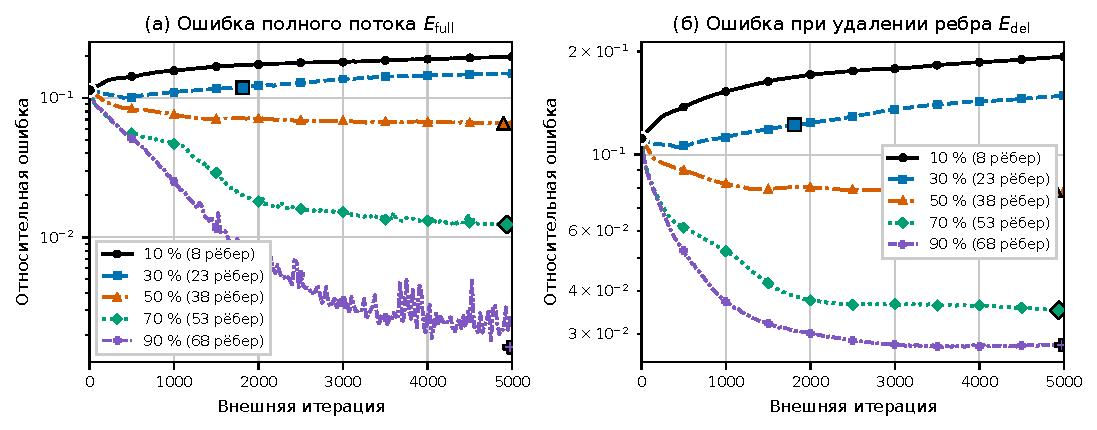
\includegraphics[width=\textwidth]{figures/exp3_random_fraction_convergence.pdf}
\caption{Зависимость качества восстановления от доли случайно наблюдаемых
рёбер: (а) относительная ошибка потока на всех 76 рёбрах исходной сети;
(б) средняя относительная ошибка потоков в 12 сетях с удалённым ребром.
Множества наблюдений вложены. Увеличенный заполненный маркер показывает
итерацию с минимальным значением целевой функции \eqref{eq:outer-objective};
линии различаются цветом, штриховкой и формой маркеров.}
\label{fig:exp3}
\end{figure}

\begin{table}[!ht]
\centering
\caption{Ошибки возвращаемой матрицы при случайном выборе наблюдаемых рёбер.}
\label{tab:exp3}
\medskip
\begin{tabular}{@{}rrrrr@{}}
\toprule
Доля, \% & Число рёбер & $k_*$ & $E_{\rm full}(D_*)$ & $E_{\rm del}(D_*)$ \\
\midrule
10 &  8 &    4 & 0.11328 & 0.11146 \\
30 & 23 & 1812 & 0.11853 & 0.12213 \\
50 & 38 & 4899 & 0.06569 & 0.07859 \\
70 & 53 & 4938 & 0.01237 & 0.03515 \\
90 & 68 & 4972 & 0.00163 & 0.02784 \\
\bottomrule
\end{tabular}
\end{table}

При 10 процентах маска содержит всего восемь потоков. Целевая функция выбирает
четвёртую итерацию: наблюдаемая невязка уменьшается на 4.0 процента, тогда как
$E_{\rm full}$ и $E_{\rm del}$ улучшаются лишь на 0.6 и 0.2 процента. К
последней итерации обе контрольные метрики существенно превышают значения в
возвращаемой точке; целевая функция также не обновляет минимум. Для
испытанной 30-процентной маски наблюдаемая невязка уменьшается на 79.8
процента, но ошибки возвращаемой матрицы выше начальных на 4.0 и 9.4 процента.
Именно второй запуск демонстрирует переобучение на наблюдаемых рёбрах.

Начиная с 50 процентов, картина меняется. Полная потоковая ошибка уменьшается
на 42.4 процента, а ошибка при удалении ребра --- на 29.6 процента. Для 70
процентов
снижение достигает 89.1 и 68.5 процента, для 90 процентов --- 98.6 и 75.1
процента. Метрика \eqref{eq:deleted-edge-error} убывает медленнее и остаётся
выше: хорошее воспроизведение исходной сети ещё не гарантирует такой же
точности после изменения множества маршрутов.

\subparagraph{Способ выбора половины рёбер}

Во второй серии число датчиков фиксировано и равно 38. Сравниваются рёбра с
наибольшими и наименьшими компонентами $\widehat f$ и независимая случайная
маска. Рис.~\ref{fig:exp4} и табл.~\ref{tab:exp4} показывают, что положение
датчиков существенно даже при одинаковом бюджете.

\begin{figure}[!ht]
\centering
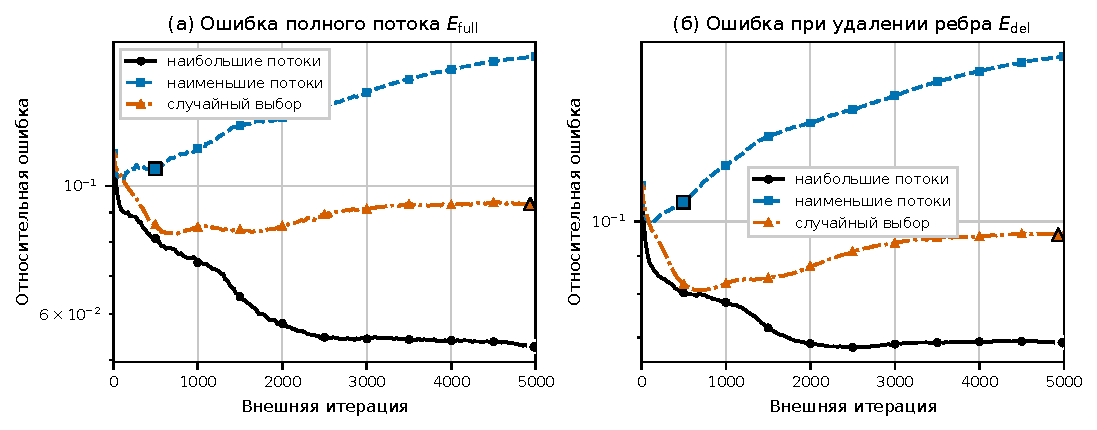
\includegraphics[width=\textwidth]{figures/exp4_selection_convergence.pdf}
\caption{Сравнение трёх способов выбрать 38 из 76 наблюдаемых рёбер:
по наибольшим референсным потокам, по наименьшим потокам и случайно.
Панели и увеличенные маркеры имеют тот же смысл, что на
рис.~\ref{fig:exp3}.}
\label{fig:exp4}
\end{figure}

\begin{table}[!ht]
\centering
\caption{Ошибки возвращаемой матрицы для трёх способов размещения 38
датчиков.}
\label{tab:exp4}
\medskip
\begin{tabular}{@{}lrrr@{}}
\toprule
Наблюдаемые рёбра & $k_*$ & $E_{\rm full}(D_*)$ & $E_{\rm del}(D_*)$ \\
\midrule
Наибольшие потоки & 4982 & 0.05271 & 0.06891 \\
Наименьшие потоки &  495 & 0.10724 & 0.10602 \\
Случайный выбор   & 4932 & 0.09312 & 0.09604 \\
\bottomrule
\end{tabular}
\end{table}

Наблюдение крупнейших потоков снижает исходные ошибки на 53.7 и 38.3
процента. Для случайной маски снижение равно 18.3 и 14.0 процента, а для
малых потоков --- лишь 5.9 и 5.1 процента. Минимум $E_{\rm full}$ не
используется при выборе решения и не обязан совпадать с $k_*$. Для малых
потоков он равен 0.10224 на итерации 67, возвращаемое значение равно 0.10724,
а на последней итерации ошибка возрастает до 0.16749. Для случайной маски
соответствующие значения равны 0.08242 на итерации 1601, 0.09312 в точке
$k_*$ и 0.09260 на последней итерации. Следовательно, правило
\eqref{eq:best-iterate} не заменяет внешнюю валидацию. В пределах данного
эксперимента рёбра с большой нагрузкой дали более информативную 50-процентную
маску, чем два других способа выбора.

\subparagraph{Доля рёбер с наибольшими потоками}

В третьей серии сравниваются вложенные маски крупнейших потоков. По мере
увеличения доли от
50 до 90 процентов обе метрики последовательно улучшаются
(рис.~\ref{fig:exp5}, табл.~\ref{tab:exp5}).

\begin{figure}[!ht]
\centering
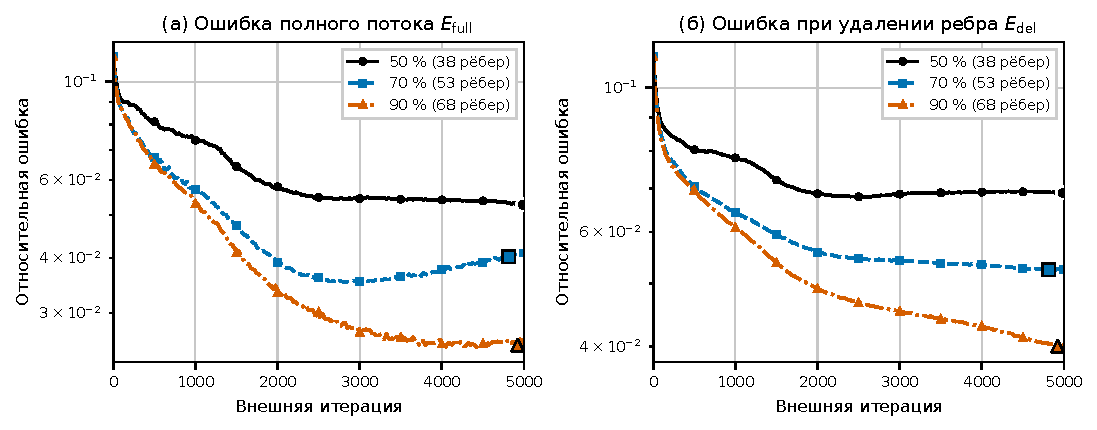
\includegraphics[width=\textwidth]{figures/exp5_top_fraction_convergence.pdf}
\caption{Зависимость качества от доли наблюдаемых рёбер с наибольшими
референсными потоками. Наблюдаемые множества вложены; обозначения панелей и
увеличенных маркеров совпадают с рис.~\ref{fig:exp3}.}
\label{fig:exp5}
\end{figure}

\begin{table}[!ht]
\centering
\caption{Ошибки возвращаемой матрицы при наблюдении рёбер с наибольшими
потоками.}
\label{tab:exp5}
\medskip
\begin{tabular}{@{}rrrrr@{}}
\toprule
Доля, \% & Число рёбер & $k_*$ & $E_{\rm full}(D_*)$ & $E_{\rm del}(D_*)$ \\
\midrule
50 & 38 & 4982 & 0.05271 & 0.06891 \\
70 & 53 & 4813 & 0.04021 & 0.05251 \\
90 & 68 & 4924 & 0.02538 & 0.04005 \\
\bottomrule
\end{tabular}
\end{table}

Относительно начальной матрицы снижение $E_{\rm full}$ составляет 53.7, 64.7
и 77.7 процента, а снижение $E_{\rm del}$ --- 38.3, 53.0 и 64.1 процента.
Однако сравнение первой и третьей серий даёт более тонкий вывод. При бюджете
50 процентов маска крупнейших потоков лучше обеих испытанных случайных масок.
При покрытии 70--90 процентов случайные маски из первой серии, напротив, дают
меньшие значения обеих метрик, чем маски крупнейших потоков той же мощности.
Это согласуется с тем,
что случайная маска сохраняет часть рёбер с малыми потоками, исключённых из
маски крупнейших потоков. Однако проведённые запуски сами по себе не доказывают
причинный механизм. Для Sioux Falls и выбранных масок стратегия ``только крупнейшие
потоки'' оказалась эффективной при бюджете 50 процентов, но не при покрытии
70--90 процентов.

\subparagraph{Идентифицируемость и ограничения эксперимента}

В Sioux Falls имеется $n(n-1)=552$ внедиагональных переменных. Маргиналии дают
не более $2n-1=47$ независимых равенств, а полный вектор потоков --- не более
76 локально независимых скалярных условий. Поэтому ранг линеаризованной
системы оставляет не менее $552-47-76=429$ неконтролируемых направлений даже
до маскирования. Это объясняет, почему относительная $L_1$-ошибка самой
матрицы не уменьшается согласованно с потоковыми ошибками: для возвращаемых
решений она находится в диапазоне 0.666--1.036 при начальном значении 0.663.
График этой величины не приводится, поскольку он не является критерием
остановки и не отражает основной прикладной результат --- качество
равновесных потоков.

Эксперимент остаётся синтетическим. В нём точно известны маргиналии и
параметры BPR, наблюдаемые потоки не содержат шума, а все вершины считаются
зонами. Кроме того, рекурсия \eqref{eq:jacobian-recurrence} игнорирует скачок
маршрутной матрицы при смене кратчайших путей. Полученные абсолютные ошибки
поэтому не следует напрямую переносить на реальную сеть. Для каждой случайной
доли проверена только одна вложенная маска, а для случайного 50-процентного
выбора во второй серии --- ещё одна маска; доверительные интервалы по маскам
не оценивались. Тем не менее единая начальная матрица, одинаковые параметры
оптимизации и две внешние диагностические метрики делают сравнение внутри
проведённых запусков согласованным.

\paragraph{Заключение}

Построен численный метод восстановления OD-матрицы по частично наблюдаемым
равновесным потокам. Внутренняя задача Бекмана решается методом
Франк--Вульфа, а маршрутные матрицы его линейных подзадач одновременно
используются для аппроксимации чувствительности потока по спросу. Внешний Adam
объединён с IPF-масштабированием, поэтому на каждой внешней итерации
восстанавливаются неотрицательность, нулевая диагональ и известные маргиналии
с заданным численным допуском.

В проведённых запусках Sioux Falls случайная маска 10 процентов дала улучшение
контрольных метрик менее 0.6 процента, а для маски 30 процентов обе ошибки
выросли. Маски 70 и 90 процентов, напротив, уменьшили $E_{\rm full}$ на 89.1
и 98.6 процента. При наблюдении половины сети рёбра с крупнейшими потоками оказались
информативнее испытанных случайной маски и маски малых потоков. Вместе с тем
при покрытии 70--90 процентов случайные маски дали меньшие ошибки, чем
маски крупнейших потоков. Во всех сценариях с заметным улучшением
$E_{\rm del}$ убывает
медленнее $E_{\rm full}$; оценка только на исходной топологии поэтому была бы
более оптимистичной.

Дальнейшее исследование должно включать шум счётчиков и маргиналий, разделение
сценариев удаления рёбер на валидационную и тестовую части, а также сравнение
с регуляризацией относительно независимой априорной OD-матрицы. Отдельная
задача состоит в выборе датчиков по чувствительности или информационному
критерию, а не только по величине потока. Наконец, требуется исследовать
устойчивость рекурсии якобиана около смены кратчайших путей и сопоставить её с
неявным дифференцированием равновесной задачи.

\begin{thebibliography}{99}

\bibitem[Beckmann et al., 1956]{Beckmann1956}
{\it Beckmann~M.~J., McGuire~C.~B., Winsten~C.~B.}
Studies in the economics of transportation.~--- New Haven: Yale University
Press, 1956.~--- 232~p.

\bibitem[Bureau of Public Roads, 1964]{BPR1964}
{\it U.S. Bureau of Public Roads.}
Traffic assignment manual for application with a large, high speed
computer.~--- Washington, DC: U.S. Department of Commerce, 1964.

\bibitem[Castiglione et al., 2021]{Castiglione2021}
{\it Castiglione~M., Cantelmo~G., Qurashi~M., Nigro~M., Antoniou~C.}
Assignment matrix free algorithms for on-line estimation of dynamic
origin--destination matrices~// Frontiers in Future Transportation.~---
2021.~--- Vol.~2.~--- Art.~640570.
DOI: 10.3389/ffutr.2021.640570.

\bibitem[Dey et al., 2020]{Dey2020}
{\it Dey~S., Winter~S., Tomko~M.}
Origin--destination flow estimation from link count data only~//
Sensors.~--- 2020.~--- Vol.~20, No.~18.~--- Art.~5226.
DOI: 10.3390/s20185226.

\bibitem[Frank, Wolfe, 1956]{FrankWolfe1956}
{\it Frank~M., Wolfe~P.}
An algorithm for quadratic programming~// Naval Research Logistics
Quarterly.~--- 1956.~--- Vol.~3, No.~1--2.~--- P.~95--110.
DOI: 10.1002/nav.3800030109.

\bibitem[Kingma, Ba, 2015]{KingmaBa2015}
{\it Kingma~D.~P., Ba~J.}
Adam: a method for stochastic optimization~// 3rd International Conference
on Learning Representations (ICLR).~--- San Diego, 2015.~--- P.~1--15.
URL: \url{https://arxiv.org/abs/1412.6980} (accessed 13.07.2026).

\bibitem[LeBlanc et al., 1975]{LeBlanc1975}
{\it LeBlanc~L.~J., Morlok~E.~K., Pierskalla~W.~P.}
An efficient approach to solving the road network equilibrium traffic
assignment problem~// Transportation Research.~--- 1975.~--- Vol.~9,
No.~5.~--- P.~309--318. DOI: 10.1016/0041-1647(75)90030-1.

\bibitem[Mohanty, Pozdnukhov, 2020]{Mohanty2020}
{\it Mohanty~S., Pozdnukhov~A.}
Dynamic origin--destination demand estimation from link counts, cellular
data and travel time data~// Transportation Research Procedia.~--- 2020.~---
Vol.~48.~--- P.~1722--1739. DOI: 10.1016/j.trpro.2020.08.209.

\bibitem[Sinkhorn, Knopp, 1967]{SinkhornKnopp1967}
{\it Sinkhorn~R., Knopp~P.}
Concerning nonnegative matrices and doubly stochastic matrices~// Pacific
Journal of Mathematics.~--- 1967.~--- Vol.~21, No.~2.~--- P.~343--348.
DOI: 10.2140/pjm.1967.21.343.

\bibitem[Transportation Networks for Research, 2026]{TNTP2026}
{\it Transportation Networks for Research Core Team.}
Transportation Networks for Research: Sioux Falls network and trip table
[Electronic resource].
URL: \url{https://github.com/bstabler/TransportationNetworks/tree/master/SiouxFalls}
(accessed 13.07.2026).

\bibitem[Yang et al., 1992]{Yang1992}
{\it Yang~H., Sasaki~T., Iida~Y., Asakura~Y.}
Estimation of origin--destination matrices from link traffic counts on
congested networks~// Transportation Research Part B: Methodological.~---
1992.~--- Vol.~26, No.~6.~--- P.~417--434.
DOI: 10.1016/0191-2615(92)90008-K.

\bibitem[Zhou, List, 2010]{ZhouList2010}
{\it Zhou~X., List~G.~F.}
An information-theoretic sensor location model for traffic
origin--destination demand estimation applications~// Transportation
Science.~--- 2010.~--- Vol.~44, No.~2.~--- P.~254--273.
DOI: 10.1287/trsc.1100.0319.

\end{thebibliography}

\end{document}
